\documentclass{standalone}
\usepackage{tikz}
\usetikzlibrary{arrows}

\begin{document}
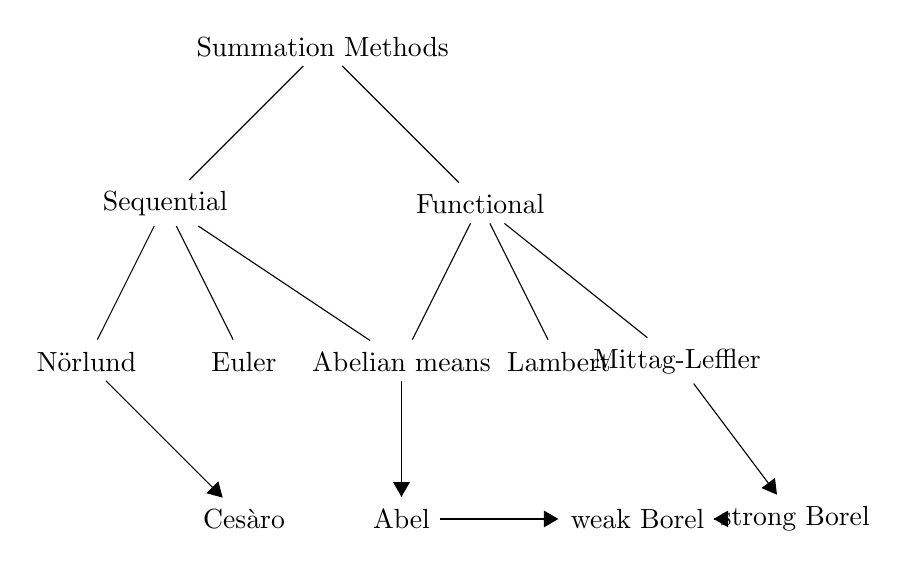
\begin{tikzpicture}[>=triangle 60, shorten >=1pt]
    \node (A) at (0,4) {Summation Methods};
    \node (B1) at (-2,2) {Sequential};
    \node (B2) at (2,2) {Functional};
    \node (C1) at (-3,0) {Nörlund};
    \node (C2) at (-1,0) {Euler};
    \node (C3) at (1,0) {Abelian means};
    \node (C4) at (3,0) {Lambert};
    \node (C5) at (4.5,0) {Mittag-Leffler};
    \node (D1) at (-1,-2) {Cesàro};
    \node (D2) at (1,-2) {Abel};
    \node (D3) at (4,-2) {weak Borel};
    \node (D4) at (6,-2) {strong Borel};

    \draw (A) -- (B1);
    \draw (A) -- (B2);
    \draw (B1) -- (C1);
    \draw (B1) -- (C2);
    \draw (B1) -- (C3);
    \draw (B2) -- (C3);
    \draw (B2) -- (C4);
    \draw (B2) -- (C5);
    \draw[->] (C1) -- (D1);
    \draw[->] (C3) -- (D2);
    \draw[->] (D2) -- (D3);
    \draw[->] (D3) -- (D4);
    \draw (C3) -- (D2); % For Abelian means to Abel
    \draw[->] (C5) -- (D4); % For Mittag-Leffler to strong Borel
    % Alternatively, using the twoheadrightarrow:
    % \draw[->>] (C5) to[bend right] (D4);
\end{tikzpicture}
\end{document}